\chapter{The Data}
A proof of concept for the proposed marketing attribution model involves its actual implementation. But in order to train and evaluate it, we first need relevant data, which is introduced in this section.\\
Beginning with an exploration of the available data, we subsequently outline necessary transformations essential for the adaptation to our conversion prediction model. 
The dataset used in this thesis is an anonymized data set from 'GetYourGuide' a German-based online travel agency. 

\section{Data Description}

The dataset consists of 1,738,080  observations documenting 7 features, with several of these touchpoint observations belonging to one customer journey.
The features, their range and description can be found in the following list:
\begin{description}
    \item[transaction:] 1 - if customer journey lead to conversion; 0 - otherwise
    \item[platform:] mobileWeb, desktop, android or ios
    \item[country\_name:] country where the touchpoint occurred    
    \item[journey\_id:] Identifying all the observations belonging to one customer/customer journey
    \item[channel\_id:] Identifying the 24 different marketing channels (Channel\_1, $\cdots$,\ Channel\_24)
    \item[timestamp:] time when the touchpoint occurred
    \item[timestamp\_conversion:] If a conversion occurred, time of this conversion, else NaN
\end{description}

A key value is given by \textbf{journey\_id} as it uniquely identifies a touchpoint with a customer which can be used to form the individual customer journeys.\\
In total there are 748,468 customer journeys, a majority only consisting of a single touchpoint, an average length of 2.322 and a maximum length of 3,143. As customer journeys of this length seem unreasonable and are impractical for implementation reasons we limit the data to the customer journeys with a length of at most 16 touchpoints which is the 0.99 percentile of customer journey lengths. Following this approach, 6,820 customer journeys with at least 17 touchpoints are eliminated leaving us with 1,514,307 observations.\\
The target value for the phased GRU network to predict is the variable \textbf{transaction}. For all customer journeys with conversion (\textit{transaction==1}), the timestamp of the conversion is recorded and can be used to identify touchpoints that happen after conversion. As those touchpoints cannot influence the previous conversion we remove another 26 touchpoints, so we effectively work with 1,514,281 touchpoints and 741.646 customer journeys of which a total of 13,506 (1.822 \% of all) customer journeys lead to conversion. 
This means that the data set is heavily unbalanced with over 98\% of customer journeys not having an observed transaction. Therefore, it's important to be careful as a classifier labeling all data as "no transaction"\ would be highly accurate without learning anything valuable from the data. How this problem is actually dealt with is further elaborated in Chapter 6 when discussing the implementation of the predictor. \\
As the value of \textbf{timestamp\_conversion} depends on the outcome it can't be used for conversion prediction and \textbf{journey\_id} shouldn't be used for prediction beyond grouping the customer journeys together, since it only serves as an identifier and contains no actual information. Therefore the next section does not consider those variables and focuses on \textbf{channels}, \textbf{country\_name}, and \textbf{platform} instead.

\begin{description}
    \item[Channels:]
\end{description}

The data set contains a total of 24 distinct marketing channels that serve as potential touchpoint avenues, which are the focal points in the MTA model. In the following paragraph a more in-depth analysis for the channels is performed.\\
\begin{figure}[h]
\centering
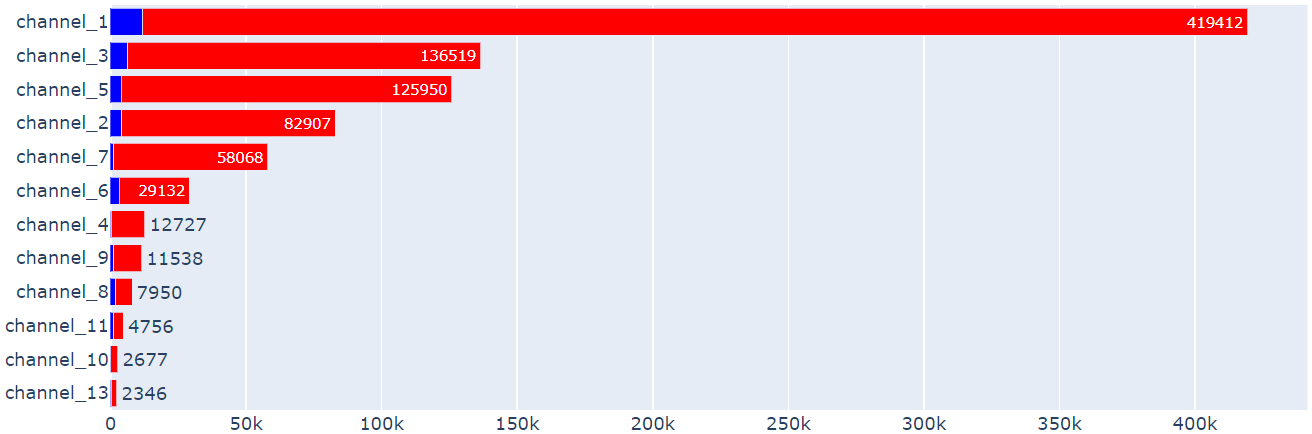
\includegraphics[width=16cm]{images/chan1.png}
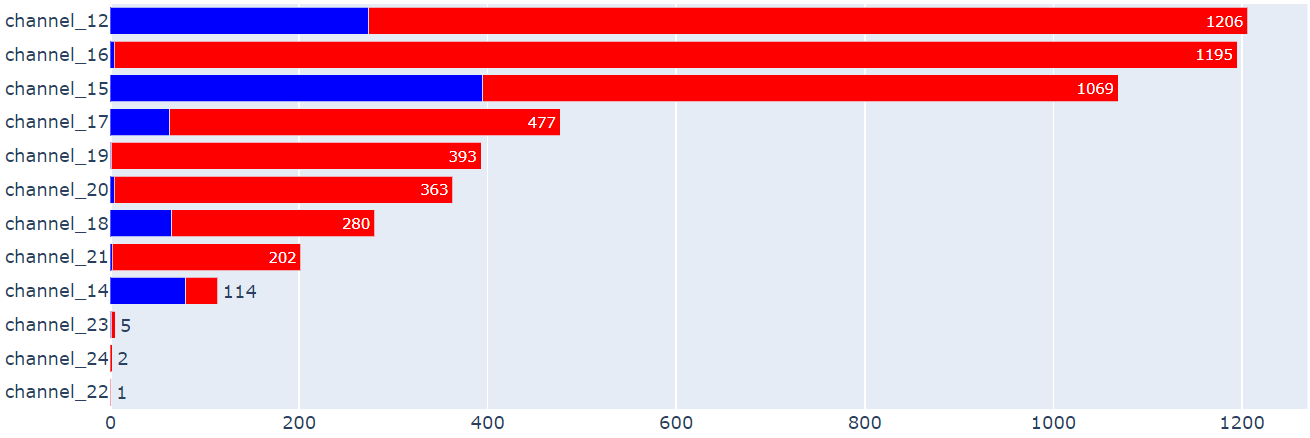
\includegraphics[width=16cm]{images/chan2.png}
\caption{Channel Occurences}
\label{fig:channel1}
\end{figure}
Upon examining the distribution of these channels across customer journeys, it becomes apparent that their occurrence does not follow a uniform pattern. Figure \ref{fig:channel1} illustrates this observation as it visualizes the number of channel occurrences across all customer journeys (not counting duplicates per customer journey) in a histogram. It's evident that some channels are encountered in only a handful of customer journeys, like channel\_22 which is only present in a single customer journey, while some other channels are remarkably prevalent, being observed several hundred thousand times.\\

Furthermore, Figure \ref{fig:channel1} divides the bars into a blue part, representing those customer journeys that ended in a transaction, and a red part representing the remaining customer journeys for which no conversion was documented. It is noteworthy that across nearly all instances, the red portion of the bars surpasses the blue counterpart with channel\_14 being the only exception there. However, it is important to highlight that for all channels the relative proportions between these two categories vary.

\begin{figure}[h]
\centering
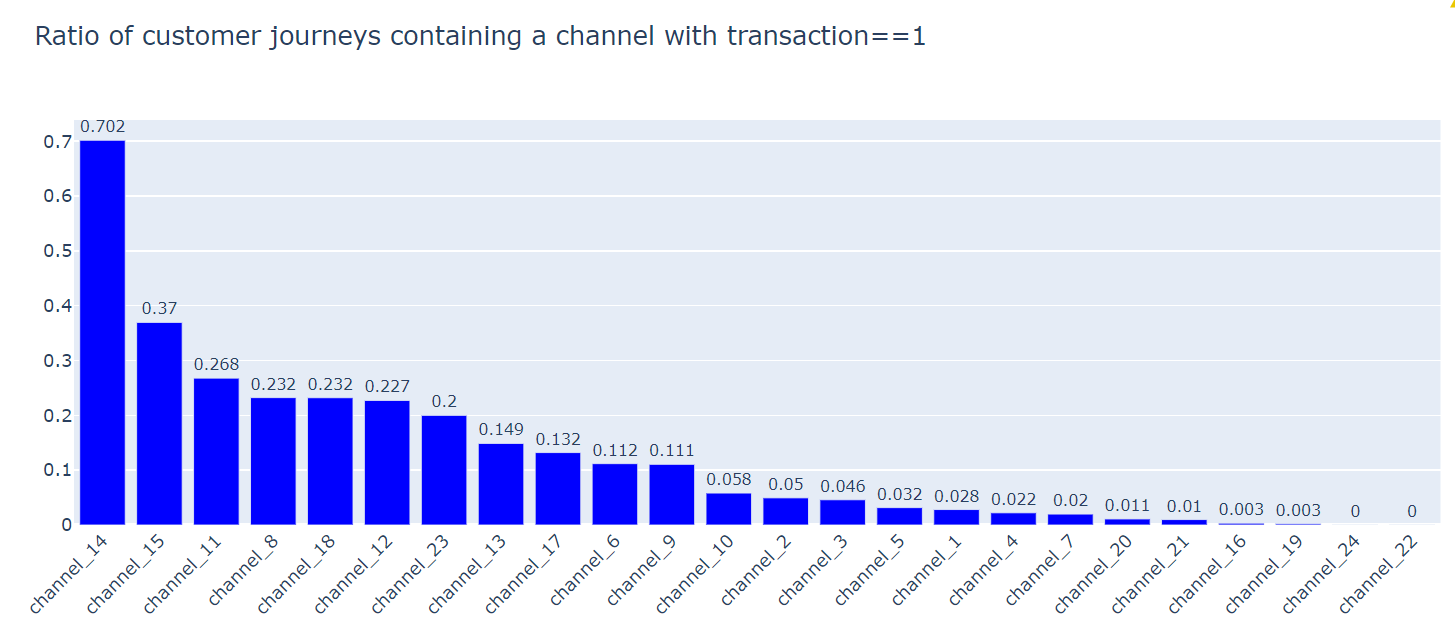
\includegraphics[height=7cm]{images/ratios_new.png}
\caption{Ratios}
\label{fig:ratio}
\end{figure}

To further explore these proportions, in Figure \ref{fig:ratio} the ratio of customer journeys containing a channel that actually led to conversion is visualized. For example of all customer journeys that contain channel\_14 around 70\% led to conversion, while of the customer journeys that contained channel\_10 only about 5\% ended with conversion. \\
As a result of the multi-touch attribution model one would expect the obtained channel importances to reflect this distribution to some extent, while also containing some differences. \\

\begin{description}
    \item[Countries:]
\end{description}
Another variable that is recorded is the country, where the customer is located. A total of 233 different countries were observed in the dataset. The location is observed for each touchpoint separately and thus does not have to stay constant within a customer journey.

\begin{figure}[h]
\centering
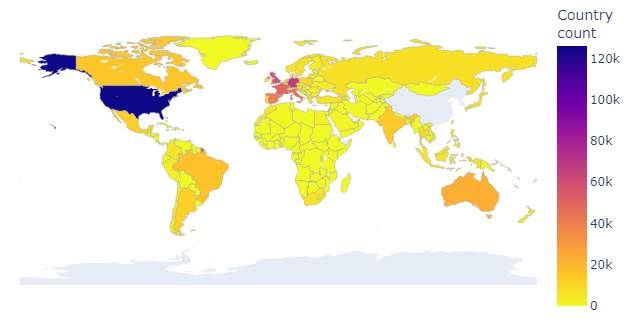
\includegraphics[height=7cm]{images/countrys.png}
\caption{Touchpoint location}
\label{fig:countrys}
\end{figure}

In Figure \ref{fig:countrys}, a visual representation of the global distribution of touchpoints is displayed. It's visible that touchpoints are dispersed worldwide, spanning from the United States to the Vatican, while China is a notable exception. This is surprising as there are offers for China on the GetYourGuide website but is probably caused by the censorship of the Internet in China and the common usage of VPN while traveling there and therefore masking China as the actual location. 
The United States boasts the highest number of touchpoints, closely followed by Western European countries, while the fewest touchpoints are found across Asia and Africa. \\
This does not represent the customer's nationality. As mentioned in the chapter introduction the data stems from an online travel agency therefore it's very possible that customers are traveling when exposed to a touchpoint.

\begin{description}
    \item[Platform:]
\end{description}
The variable \textbf{platform} holds information on the devices the touchpoint recorded on. The four possible expressions for this feature are \textit{mobileWeb}, \textit{desktop}, \textit{android}, and \textit{ios}.  

\begin{figure}[h]
\centering
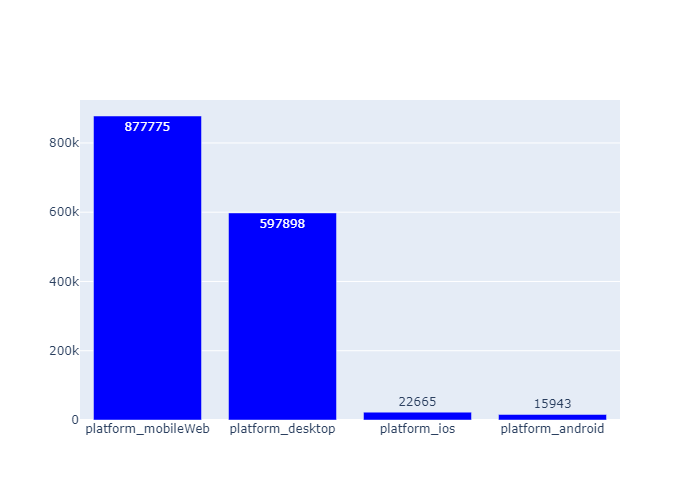
\includegraphics[height=7cm]{images/platforms.png}
\caption{Platform}
\label{fig:plattform}
\end{figure}

In this Histogram \ref{fig:plattform} one can observe two groups forming. \textit{mobileWeb} and \textit{desktop} are both in a similar range and together represent the majority of all touchpoints. On the other hand \textit{ios} and \textit{android} are also in a similar range but together only represent around 2.5\% .\\

With the available features we have no information on the customers or any other brand interactions such as click events, therefore no causal model could be implemented for this data. 

\section{Data Transformation}

The data set previously has been used for a different MTA approach, and thus some transformation is necessary to make it compatible with the phased GRU network. 
In the previous section already some changes to the data set were established with which we continue to work. 
Even though we said to remove the \textit{journey\_id} we will still use it for the transformation as an identifier in this section. 
The first transformation is to create dummy variables for the categorical variables \textit{channel, platform} and \textit{country\_name}. A dummy variable is created by replacing the variable column with columns for each possible expression of this variable. Each of these newly created columns is assigned '1' if a given observation expressed the respective categorical value and '0' else.\\
This greatly expands the size of the data set but is the best way to handle categorical data, that can not easily be transformed in an ordinal way. \\
The next transformation is to group together all touchpoints belonging to the same customer in order to form individual customer journeys. Previously the format of the dataset was in a table format \textit{touchpoint $\times$ features} where each row corresponds to a touchpoint observation with the observed features in the columns and the customer journeys aren't apparent. 
For the GRU network, we want to use customer journeys grouped together as one observation, which adds another dimension \textit{customer $\times$ touchpoints $\times$ features}. So for each customer $c$ with a customer journey of length $L$, we get $x_c=( f_l^T, t_l)_{l=1\cdots, L}$, where $f_l$ collects the recorded features of the $l$-th touchpoint, $t_l$ the timepoint of this touchpoint. We deliberately put the timestamp in the last position of the created tensor in order to extract the time by simply accessing the last position using the index "\textit{-1}". These timestamps are then used for the time gate. 
A problem that emerges with this approach are the varying customer journey lengths. While ragged tensors exist and could be used here to create tensors with an unspecified dimension size, ragged tensors are not very practical and cannot be used efficiently as of today. 
In an article \cite{patton-2022} presented an example that illustrates, that while using ragged tensors he was able to achieve marginally improved results but the computations for each training epoch took around 60 times more time compared to the same model trained with padded input. 
Therefore we also use padded input data, meaning all customer journeys get filled up with zeros to achieve the same length of 16. Here the decision to exclude long customer journeys proves to be helpful, as we don't have to artificially inflate the data set in order to keep all 3,143 touchpoints of the longest customer journey. \\
As target value, we use $y_c\in\{0,1\}$, the \textbf{transaction} for each customer which identifies two classes the successful and unsuccessful customer journeys. Therefore our prediction task is in fact a classification problem and we need to predict the class once per customer journey, at the end, when all touchpoints are considered. \\
The whole data is then split into a training and a test data set to appropriately fit and evaluate the model. 75 percent of customer journeys are randomly selected as training data in order to allow the model to learn well. 
The remaining 25 percent of the data is used to evaluate the predictions of the model after training is done. \\
Finally the data is split into batches of a fixed size to not overstrain storage space and achieve a faster training speed.\\
